\chapter{Теоретический раздел}

\section{Алгоритм Хаффмана}

Пусть $A={a_1,a_2,…,a_n}$ — алфавит из $n$ различных символов, $W={w_1,w_2,…,w_n}$ — соответствующий ему набор положительных целых весов. Тогда набор бинарных кодов $C={c_1,c_2,…,c_n}$ , где $c_i$ является кодом для символа $a_i$, такой, что:

\begin{itemize}
\item $c_i$ не является префиксом для $c_j$, при $i\neq j$,
\item cумма $\sum_{i \in [1,n]}{w_i \cdot |c_i|}$ минимальна ($|c_i|$ — длина кода $c_i$).
\end{itemize}
называется кодом \textbf{Хаффмана}.

\section{Алгоритм построения бинарного кода Хаффмана}

Построение кода Хаффмана сводится к построению соответствующего бинарного дерева по следующему алгоритму:
\begin{enumerate}
\item Составим список кодируемых символов, при этом будем рассматривать один символ как дерево, состоящее из одного элемента c весом, равным частоте появления символа в строке.
\item Из списка выберем два узла с наименьшим весом.
\item Сформируем новый узел с весом, равным сумме весов выбранных узлов, и присоединим к нему два выбранных узла в качестве детей.
\item Добавим к списку только что сформированный узел вместо двух объединенных узлов.
\item Если в списке больше одного узла, то повторим пункты со второго по пятый.
\end{enumerate}

Рассмотрим на примере.

Закодируем слово \textbf{abracadabra}. Тогда алфавит будет $A={a,b,r,c,d}$, а набор весов (частота появления символов алфавита в кодируемом слове) $W={5,2,2,1,1}$. В дереве Хаффмана будет 5 узлов:

\begin{table}[H]
\begin{tabular}{|l|l|l|l|l|l|}
\hline
Узел & a & b & r & c & d \\ \hline
Вес  & 5 & 2 & 2 & 1 & 1 \\ \hline
\end{tabular}
\end{table}

По алгоритму возьмем два символа с наименьшей частотой — это c и d. Сформируем из них новый узел cd весом 2 и добавим его к списку узлов:

\begin{table}[H]
\begin{tabular}{|l|l|l|l|l|}
\hline
Узел & a & b & r & cd \\ \hline
Вес  & 5 & 2 & 2 & 2  \\ \hline
\end{tabular}
\end{table}

Затем опять объединим в один узел два минимальных по весу узла — r и cd:

\begin{table}[H]
\begin{tabular}{|l|l|l|l|}
\hline
Узел & a & b & rcd \\ \hline
Вес  & 5 & 2 & 4   \\ \hline
\end{tabular}
\end{table}

Еще раз повторим эту же операцию, но для узлов rcd и b:

\begin{table}[H]
\begin{tabular}{|l|l|l|}
\hline
Узел & a & brcd \\ \hline
Вес  & 5 & 6    \\ \hline
\end{tabular}
\end{table}

На последнем шаге объединим два узла — brcd и a:

\begin{table}[H]
\begin{tabular}{|l|l|}
\hline
Узел & abrcd \\ \hline
Вес  & 11    \\ \hline
\end{tabular}
\end{table}

\begin{figure}[h!]
            \centering
            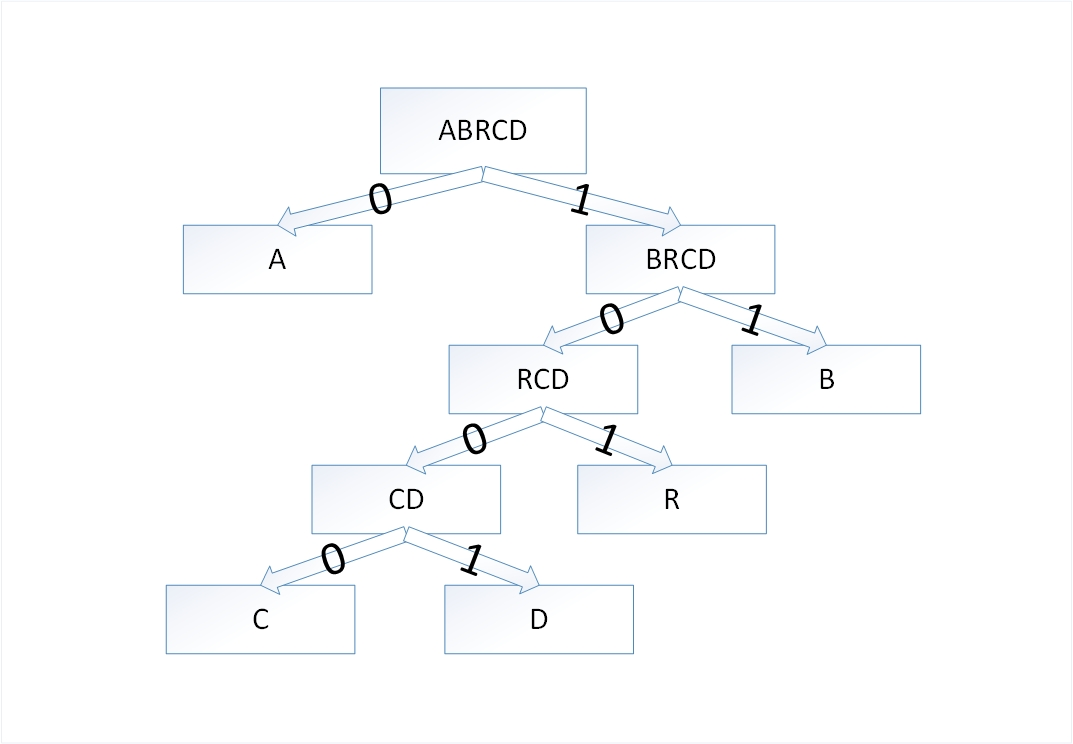
\includegraphics[scale=0.5]{assets/huffman.jpg}
            \caption{Дерево Хаффмана}
            \label{img:1}
        \end{figure}

Остался один узел, значит, мы пришли к корню дерева Хаффмана. Теперь для каждого символа выберем кодовое слово (бинарная последовательность, обозначающая путь по дереву к этому символу от корня):

\begin{table}[H]
\begin{tabular}{|l|l|l|l|l|l|}
\hline
Символ & a & b  & r   & c    & d    \\ \hline
Код    & 0 & 11 & 101 & 1000 & 1001 \\ \hline
\end{tabular}
\end{table}

Таким образом, закодированное слово abracadabra будет выглядеть как 01110101000010010111010. Длина закодированного слова — 23 бита. Стоит заметить, что если бы мы использовали алгоритм кодирования с одинаковой длиной всех кодовых слов, то закодированное слово заняло бы 33 бита, что существенно больше.

Поскольку ни один из полученных кодов не является префиксом другого, они могут быть однозначно декодированы при чтении их из потока. Кроме того, наиболее частый символ сообщения A закодирован наименьшим количеством битов, а наиболее редкий символ D и C – наибольшим.

Классический алгоритм Хаффмана имеет один существенный недостаток. Для восстановления содержимого сообщения декодер должен знать таблицу частот, которой пользовался кодер. Следовательно, длина сжатого сообщения увеличивается на длину таблицы частот, которая должна посылаться впереди данных, что приводит к увеличению размеров выходного файла. Кроме того, необходимость наличия полной частотной статистики перед началом собственно кодирования требует двух проходов по сообщению: одного для построения модели сообщения (таблицы частот и дерева), другого для собственно кодирования.